\documentclass[letterpaper, 12 pt, conference]{ieeeconf}

\IEEEoverridecommandlockouts
% This command is only needed if 
% you want to use the \thanks command

\overrideIEEEmargins
% Needed to meet printer requirements.
%\usepackage[margin=0.65in]{geometry}

% See the \addtolength command later in the file to balance the column lengths
% on the last page of the document

% The following packages can be found on http:\\www.ctan.org
\usepackage{graphics} % for pdf, bitmapped graphics files
\usepackage{epsfig} % for postscript graphics files
\usepackage{mathptmx} % assumes new font selection scheme installed
\usepackage{times} % assumes new font selection scheme installed
\usepackage{amsmath} % assumes amsmath package installed
\usepackage{amssymb}  % assumes amsmath package installed

\usepackage{hyperref}
\usepackage{url}
%\usepackage[pdftex]{graphicx}
%\usepackage{amsfonts}
\usepackage{subfigure} 
\usepackage{algorithm}
%\usepackage{algorithmic}
\usepackage{algcompatible}
\usepackage{framed}
\usepackage{balance}
\graphicspath{{images/}}
\usepackage{multicol}

\title{\LARGE \bf
Generating Natural Language Descriptions of Trajectories Using Long Short Term Memory Neural Networks}

\author{Rodolfo Corona and Rolando Fernandez}

\begin{document}

\maketitle
\thispagestyle{empty}
\pagestyle{empty}

\section{Problem Description}

Given a point-cloud $p$ $\in$ $P$ and a manipulation trajectory $t$ $\in$ $T$, our goal is to output a free-form  Natural Language (NL) description $l$ $\in$ $L$ that describes the trajectory $t$:

\begin{equation}
f: T\times P \mapsto L
\end{equation}

\section{Hypothesis}

Given $(t,p)\in T\times P$, a Long Short Term Memory (LSTM) neural network architecture may be trained to sequentially generate NL descriptions that accurately describe the actions the agent performs under a trajectory $t$ $\in$ $T$.

\section{Background}

\subsection{LSTMs}

LSTMs are a variant of the Recurrent Neural Network (RNN) architecture which attempt to alleviate the vanishing gradient problem which traditional RNNs can suffer from. 
\par
LSTMs accomplish this through the use of \textit{gates}, which change the cell's state at each time step based on the current time step's input and the last time step's output. Intuitively, at each time step, an LSTM cell decides which information to forget and which new information to incorporate through the use of its gates. Formally, this computation takes the form of the following gate update equations: 

\begin{align}
f_t &= \sigma (W_fx_t + U_fh_{t-1}+b_f) \\
i_t&=\sigma (W_ix_t + U_ih_{t-1}+b_i) \\
c_t &= tanh (W_cx_t  + U_c h_{t-1}+b_c) \\
o_t &= \sigma (W_o x_t + U_o h_{t-1} + b_o)
\end{align}

And the cell state update and output equations:

\begin{align}
C_t &= f_tC_{t-1}+ i_t c_t \\
h_t&= o_t \cdot tanh(C_t)
\end{align}
Where $\sigma$ is the sigmoid function and, given a gate $g$, $b_g$ is the bias and $W_g$ and $U_g$ are the input and hidden state weight matrices respectively \cite{hochreiter1997long}.  

\subsection{Robobarista}

Sung et al. utilized the Robobarista framework to perform an experiment investigating whether it would be possible for a robotic agent to learn to manipulate novel objects through the use of deep multimodal embeddings.

The modalities used  by Sung et al. were point clouds, NL descriptions, and trajectories. The purpose of the experiment was to determine whether point clouds and NL descriptions could be mapped to trajectories, as shown in Equation (\ref{eq:robobarista}). 

\begin{equation}\label{eq:robobarista}
f: P\times L \mapsto T
\end{equation}

Sung et al. developed a system for generalizing manipulation planning based on the fact the the objects which an agent would need to manipulate share many similar object parts to such as ‘handles’, ‘triggers’, and ‘buttons’. Sung et al. proposed that through the use of natural language descriptions for the actions to be performed the agent would be able generalize manipulation trajectories to different objects with similar parts to be manipulated \cite{sung2016robobarista}. 

Our work differs from that of Sung et al. by seeking to perform the inverse of the mapping in Equation (\ref{eq:robobarista}), which is to generate novel NL descriptions for $(t,p)\in T\times P$. We seek to create a system that gives an agent the ability to explain the actions it will take or that need to be performed to complete a given task. This system would give an agent the ability to generate explanations for the manipulation tasks that it is performing, allowing humans to better understand the actions and decisions taken by the agent.


\section{Related Work}

\subsection{LSTMs}

LSTMs have been successfully applied to a variety of sequence-to-sequence tasks such as machine translation \cite{sutskever2014sequence} and handwriting synthesis \cite{graves2013generating}. These problems are generally approached by using an LSTM encoder-decoder architecture, which consists of an LSTM encoder which takes an input sequence and generates a vector representation of it. This representation is then used to condition an LSTM decoder which generates a sequence of data in the output modality of the given domain. The use of the encoder-decoder scheme allows for sequences of varying and arbitrary lengths to be mapped to each other. 

Closest to our work, and a source of motivation behind it, is that of Venogupalan et al. \cite{Venugopalan_2015_ICCV}, which uses LSTMs to generate natural language descriptions of videos.  

\subsection{Explainable AI}

There has been relatively little work done in systems which generate natural language descriptions of their internal state and decisions. Johnson et al. describe a fighter pilot simulation system which can generate explanations for the decisions that the agent took. Their work, however, uses scripted responses and a rule-based system to decide which to use. Similarly, there have been works which use templates to generate explanations. Wang et al. present a system which generates explanations for an agent's POMDP model using natural language \cite{wang2016trust}. Lomas et al. also present a system which allows a system to explain its actions using natural language templates when queried by a human \cite{lomas2012explaining}. These explanations, however, are not generalizable to situations which their templates do not cover. In contrast, our work attempts to generate descriptions in a more robust manner by using a generative LSTM model. 

\section{Methods}

\subsection{Robobarista Dataset}

Using the Robobarista framework, Sung et al. \cite{sung2016robobarista} collected a dataset consisting of triplets of the form $(t, p, l)$. The dataset consists of 116 objects with 249 parts (i.e. 249 point cloud segments) along with 250 NL instructions, for which 1225 manipulation trajectories were collected. 

Each of the 116 objects is split into parts depending on the number of NL instructions that pertain to it and the original point cloud scene is segmented with respect to the part frames, being stored as a Comma Separated Value (CSV) file consisting of [x,y,z,r,g,b] values. 

Furthermore, each of the objects have multiple manipulation trajectories for each part stored as a list of waypoints. Waypoints are encoded in tuples $\{g, t_x, t_y, t_z, r_x, r_y, r_z, r_w\}$, where $g\in \{``open", ``closed", ``holding"\}$ denotes the gripper status of the PR2 robot which they used, $(t_x, t_y, t_z)$ denotes translation, and $(r_x, r_y, r_z, r_w)$ denotes rotation in quaternions. 

For our experiments, we split the dataset into 5 folds of train and test data in order to perform 5-fold cross validation.

\subsection{METEOR Evaluation}

In order to evaluate the efficacy of all of our models, we used the sentence comparison package METEOR \cite{Denkowski14meteoruniversal}. METEOR is a framework used to evaluate sentence similarities through word alignment. Word alignment is scored on metrics such as exact matches, shared word stems, and synonymy in the WordNet \cite{kilgarriff2000wordnet}. The motivation behind the evaluation metrics is to score how similar two sentences are in phrasing, word choice, and semantics. 

\subsection{Baseline with Point Clouds}\label{baseline_pc}

For our initial baseline, we created a pipeline that utilizes the point clouds in the Robobarista dataset to perform inference using K-Means clustering and K-Nearest Neighbors (Figure \ref{fig:Baseline_Point_Cloud}). 

We first train a K-Means model and a KNN model using the training data for each of the 5 folds. The point cloud key points are taken from the segmented object part point cloud CSV files. We create two vectors from the CSV files, one is a vector $\overline{P}$ of all the point clouds in the training set where the point clouds themselves are vectors of key points and the other is a vector $K$ of all the key points in the training set. 

Utilizing the K-Means algorithm in the Python SKLearn package, we cluster the key points in $K$ into 50 clusters and get back a trained K-Means model. With the K-Means model, we extract a cluster prediction for each key point in each individual point cloud in $\overline{P}$. Then, using the cluster predictions as in \cite{csurka2004visual}, we compute a Bag of Features (BOF) vector for each point cloud based on the number of occurrences of each cluster.

The BOF vectors are then used as input with to the K-Nearest Neighbors classifier in the Python SKLearn package and in return we get a trained KNN model. We are then able to use this KNN model to determine the nearest neighbor of a given point cloud. 


\begin{figure}[htb!]
  \centering
  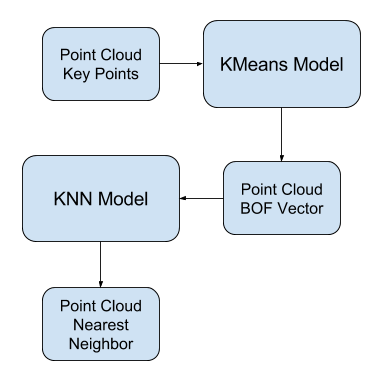
\includegraphics[width=0.3\textwidth]{Baseline-Point_Cloud}
  \caption{Baseline model with Point Clouds}
  \label{fig:Baseline_Point_Cloud}
\end{figure}

\subsection{Baseline Validation}

In order to determine the best cluster count to utilize for the baseline experiments we conducted a set of validation experiments by incrementing cluster counts and evaluating on the validation set for each fold in the dataset. Using our initial cluster count of $50$ as the starting count, we evaluated $6$ other cluster count values by incrementing by $50$ until we reached a cluster count of $350$ for a total of $7$ cluster counts to test. 

The $7$ cluster counts were used to train a K-Means model and a K-Nearest Neighbor model as described in Section \ref{baseline_pc}. The trained models were then evaluated on the validation data of the $5$ folds in the dataset. Following this, the METEOR scores for each of the $5$ folds were averaged for each of the $7$ cluster counts with the highest average being the cluster count that is used in our final Baseline experiments (Table \ref{baseline_validation_table}).

\begin{table}
\center
\begin{tabular}{|c|c|}
\hline
\textbf{Cluster Count} & \textbf{Average Score} \\
\hline
50 & 0.111828 \\
\hline
100 & 0.091469 \\
\hline
150 & 0.095311 \\
\hline
200 & 0.098440 \\
\hline
250 & 0.097979 \\
\hline
300 & 0.098583 \\
\hline
350 & 0.097280 \\
\hline
\end{tabular}
\caption{The average scores over the 5 folds for each of the $7$ cluster count values for the validation data of the dataset.}\label{baseline_validation_table}
\end{table}

\subsection{Baseline with Point Clouds and Trajectories}

For our second baseline, we created a pipeline which subsumes the first by utilizing both the point clouds and trajectories in the Robobarista dataset to perform inference using K-Means clustering and K-Nearest Neighbors (Figure \ref{fig:Baseline_Point_Cloud_and_Trajectories}). 

We first train a K-Means model with the cluster count determined in the baseline validation experiments ($50$ clusters). The K-Nearest Neighbor model is then trained and the computed BOF point-cloud vectors are again used as input values for the K-Nearest Neighbors classifier from the SKLearn Python package. We are then able to use the trained KNN model to determine the $10$ nearest neighbors of a given pair $(t,p)\in T\times P$. We then re-rank the $10$ neighbors based on a comparison of their trajectories to that of the given trajectory using a Dynamic Time Warping (DTW) metric as suggested in \cite{chen2013dynamic}. The neighbor that receives the highest DTW score is then used to generate a NL description as in the first baseline.

\begin{figure}[htb!]
  \centering
  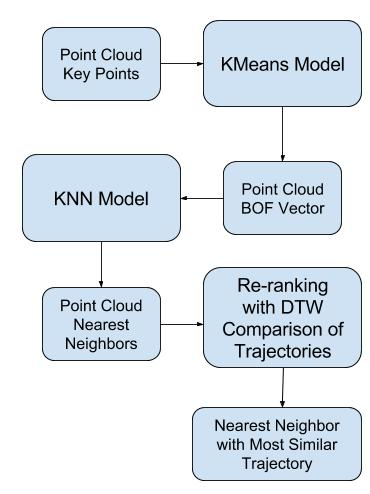
\includegraphics[width=0.3\textwidth]{Baseline-Point_Cloud_and_Trajectories}
  \caption{Baseline model with Point Clouds and Trajectories}
  \label{fig:Baseline_Point_Cloud_and_Trajectories}
\end{figure}

\subsection{LSTM Implementation}

We initially implemented an encoder-decoder LSTM neural network architecture which operated exclusively on trajectories. Specifically, our architecture used one LSTM layer to encode the inputted sequence of trajectory waypoints $t$ into an embedding $h$. This embedding was then fed into another LSTM layer which decoded it into a sequence of words $l$. A diagram representing the model may be seen in Figure \ref{fig:LSTM_diagram_1}.

\begin{figure}[h]
\center
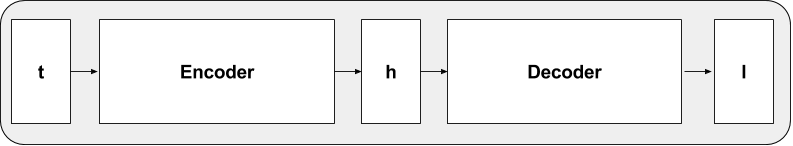
\includegraphics[scale=0.3]{Trajectory_LSTM}
\caption{Our unimodal trajectory LSTM. $t$ represents a trajectory waypoint sequence, $h$ represents the embedding generated by the encoder, and $l$ is the word sequence generated by the decoder.}
\label{fig:LSTM_diagram_1}
\end{figure}

Because point-clouds in our input were single data points, rather than sequences, we did not require an LSTM encoder to use them in our pipeline. Instead, we used the K-Means model from our baseline in order to generate a BOF vector for each point-cloud. Therefore, for our multimodal LSTM architecture, we continue to use an encoder exclusively for trajectories, and concatenate the trajectory embedding to the point-cloud BOF vector, the result of which is fed into an LSTM decoder. A diagram of our multimodal architecture may be seen in Figure \ref{fig:multimodal_LSTM}.

\begin{figure}[h]
\centering
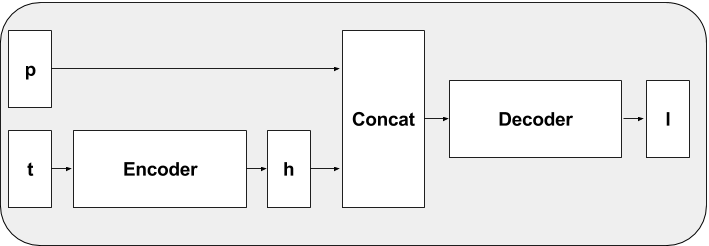
\includegraphics[scale=0.33]{Tuple_LSTM}
\caption{The architecture of our multimodal LSTM model. The model uses a trajectory encoder to generate an embedding $h$, which is concatenated with a BOF vector for a point cloud. This resulting vector is then fed to a decoder LSTM in order to generate word sequences for our phrases.}
\label{fig:multimodal_LSTM}
\end{figure}

To implement both architectures, we use the Keras\footnote{https://keras.io/} library with a TensorFlow\footnote{https://www.tensorflow.org/}. 

\subsection{Preprocessing}
After analyzing the Robobarista dataset, it was found  that the longest trajectory consisted of 18 waypoints. Therefore, all trajectories were fitted into tensors of 18 waypoints, with zero vectors used to pad trajectories of length less than 18. 
\par
Similarly, it was found that all phrases in the dataset consisted of less than 18 words. Accordingly, each phrase was converted into a tensor consisting of 18 one-hot vectors of dimensionality $|V|$, where $|V|$ is the size of the training set vocabulary for a given fold.

\subsection{LSTM Training and Tuning}

The unimodal LSTM architecture consisted of 50 hidden units in both the encoder and decoder. We trained the network over 1000 epochs with a batch size of 80, a mean squared error loss function, and RMSProp optimizer with a learning rate of 0.001.

We initially tested the multimodal LSTM with the same parameters of the original architecture, although it was found that performance dropped, something which motivated tuning of the hyperparameters in our model. Motivated by \cite{bergstra2012random}, we conducted a random search in which we trained LSTM models with randomly set values, the ranges of which may be seen in Table \ref{fig:hyperparameter_ranges}. 

\begin{table}[h]
\center
\begin{tabular}{|c|c|}
\hline
\textbf{Hyperparameter} & \textbf{Range} \\
\hline
Layers & 1 - 3 \\
\hline
Hidden Units & 25 - 200 \\ 
\hline
Dropout  & 0.0 - 0.5 \\
\hline
Training Epochs & 10 - 500 \\
\hline
Training Batch Size & 1 - 100 \\
\hline
Learning Rate & 0.001 - 1.0 \\
\hline
\end{tabular}
\caption{The ranges for each hyperparameter in our architecture over which a random search was conducted. Hyperparamters pertaining to network layers (e.g. dropout) were individually sampled for each layer in both our encoder and decoder LSTMs.}\label{fig:hyperparameter_ranges}
\end{table}

In order to mitigate computational cost, each randomly generated model was tested on only one of the 5 folds in our validation set, which itself was randomly chosen each time. In total, we trained 493 LSTMs and chose the best performing architecture for evaluation on the test set. The configuration of our best performing model may be seen in Table \ref{fig:hyperparameter_choice}.

\begin{table}[h]
\center
\begin{tabular}{|c|c|c|}
\hline
\textbf{Hyperparameter} & \textbf{Encoder} & \textbf{Decoder} \\
\hline
Layers & 3 & 2\\
\hline
Hidden Units & $94,34,49$ & 141, 18\\ 
\hline
Dropout  & 0.22, 0.11 & 0.28 \\
\hline
\end{tabular}
\begin{tabular}{|c|c|}
\hline
\textbf{Hyperparameter} & \textbf{Value} \\
\hline
Training Epochs & 320 \\
\hline
Training Batch Size & 52\\
\hline
Learning Rate & 0.001\\
\hline
\end{tabular}
\caption{The hyperparameter values pertaining to our best performing architecture. Note that dropout was only applied between hidden layers and not after output layers.}\label{fig:hyperparameter_choice}
\end{table}

\subsection{LSTM Testing}

During testing, we first generate a BOF vector for a given point-cloud. Following this, we feed both the point-cloud BOF vector and the given trajectory tensor to our network, which then generates a sequence of one-hot vectors for phrases. Because every phrase in our dataset ends with a ``." token, we generate phrases of 18 tokens and prune them past the first appearance of the ``." token.  


\section{Results}

\subsection{Baseline with Point Clouds}\label{baseline_with_point_clouds}

For the baseline, we conducted experiments using the data from each of the 5 folds, running a total of 5 trials. For each trial we created a gold reference consisting of the already known NL descriptions for each of the point clouds and a test reference consisting of the NL description returned by using the trained K-Means and KNN models.

Each point cloud in the fold test data is first inputted in the K-Means model to extract the BOF vector representation, then the BOF vector is inputted into the KNN model to retrieve the nearest neighbor of the point cloud. Lastly, we look up the NL description for the given neighbor, which is used as the output for the model. With the completed test and gold reference files we are then able to compute METEOR scores to evaluate the accuracy of our baseline.

On average the baseline performed poorly, only reaching its highest performance in the first fold achieving a final METEOR score of 0.172. Figure \ref{fig:baseline_fold_1} shows the alignment results for four sentences from the Fold 1 test set. These results were expected as the baseline only performs a simple look-up based on nearest neighbor inference from the training set point clouds and is not able to generalize properly to the test set.

\subsection{Baseline with Point Clouds and Trajectories}

For the baseline with trajectories, we conducted experiments in the same manner as described in Section \ref{baseline_with_point_clouds} using the test data from each of the 5 folds, running a total of 5 trials. For each trial we created a gold reference as well as a test reference consisting of the NL description returned by using the trained K-Means and KNN models, with the re-ranking of the $10$ nearest neighbors using a DTW Metric.

On average the baseline with trajectories still performed poorly overall, only reaching its highest performance in the first fold achieving a final METEOR score of 0.205. Though this baseline with trajectories did perform better the the baseline that only used trajectories, as seen in Figure \ref{fig:baselines_fold_1_score}. Figure \ref{fig:baseline_w_traj_fold_1} shows the alignment results for four sentences from the Fold 1 test set. When compared with Figure \ref{fig:baseline_fold_1}, we can see that at times the baseline with trajectories performed better and at others it performed worse than the baseline with only point clouds. These results were expected as this baseline with trajectories still only performs a simple look-up based on nearest neighbor inference from the training set point clouds with the added re-ranking of trajectories using a DTW metric and is still not able to generalize properly to the test set.

\subsection{LSTM Implementation}

Similarly to the baseline, both LSTM architectures was evaluated using 5-fold cross validation. The results for each fold as well as the averages over all folds were computed for all models tested, the results of which may be seen in Table \ref{fig:score_table}. It was found that the trajectory LSTM performed marginally better than all other models. Further, it may be observed that the multimodal LSTM model experienced the worst performance. To analyze the significance of the results, Student's unpaired t-tests were performed which showed that the results were not statistically significant with p-values $> 0.05$.

An illustrative example of the performance of the LSTM models may be seen in figure \ref{fig:lstm_alignment} (the alignment key is in figure \ref{fig:baseline_fold_1}). In the example, the unimodal LSTM manages to correctly infer that the trajectory pertains to pushing a button, but is unable to recognize that it is a ``white grape juice" button. Interestingly, the multimodal LSTM seems to recognize the scene and task exactly, but fails to reach full accuracy due to generating the token ``button" twice. 

\begin{table}[h]
\center
\begin{tabular}{|c|c|c|c|c|c|c|}
\hline
\textbf{Model} & \textbf{Average METEOR Score} \\
\hline
\textbf{Baseline (P)} & 0.144 \\
\hline
\textbf{Baseline (P + T)} & 0.153 \\
\hline
\textbf{LSTM (T)} & 0.155 \\
\hline
\textbf{LSTM (T + P)} & 0.132 \\
\hline
\end{tabular}
\caption{Average METEOR score per model over 5-fold cross validation. P denotes point-cloud inclusion and T denotes trajectory inclusion.}\label{fig:score_table}
\end{table}

Further, the score distributions over phrases may be seen in Figure \ref{fig:fold_1_score_lstms}. It may be observed that the unimodal LSTM experienced a smoother decrease in the number of phrases for each range of scores. Interestingly, the multimodal LSTM experienced a jump in the number of phrases on which it received a METEOR score between 0.3 and 0.4. 

\section{Difficulties}\label{Difficulties}

One of the major difficulties we encountered was that we were not able to receive a complete trained model for the work performed by Sung et al. \cite{sung2016robobarista}. To overcome the lack of the trained model for our baseline experiments, we decided to use Dynamic Time Warping (DTW) to compare trajectories that are associated with the point clouds in order to re-rank the pairs.

Additionally, we discovered while developing our baseline experiments that the segmented points clouds for each object part are not stored in the typical Point Cloud Data (PCD) format, but instead are stored in a CSV format where each point cloud point is represented as a list of values [x,y,z,r,g,b]. To deal with this unexpected format we decided to forgo the use of NARF \cite{steder2010narf} descriptors and instead considered each point in the segmented point clouds as a key point for use in the BOF representation using the K-Nearest Neighbors method. We believe that this is a fair assumption since the point clouds were segmented in order to include only the pertinent parts of each point cloud for the given trajectories. 
\par
One final difficulty we encountered was that the eldar GPU UTCS machines do not currently have the most current version of TensorFlow or Keras installed. We were eventually able to run our code on the machines through the use of Python virtual environments. Additionally, due to the size of our dataset, we found that our models train fairly quickly (in one to two hours) using CPUs, which allowed us to use the general computing clusters for our work, rather than GPU-enabled machines. 

\section{Discussion}\label{Discussion}

We believe that our current results show some promise for the validity of our hypothesis, although it is still ambiguous. Even though both baselines currently outperform our multimodal LSTM architecture, it is important to note that they both perform a simple retrieval of phrases in our training set, which means that their performance is strictly not generalizable. Therefore, we believe that the comparable performance of our LSTM models shows promise, particularly since our unimodal LSTM model experienced the best performance. 

Some examples of output from our multimodal LSTM architecture may be seen in Table \ref{fig:LSTM_examples}. From these examples, we can begin to dissect the types of problems that our current model experiences, which may be addressed in future work. For example, it may be noted that the model has a tendency to repeat certain words in its generated sequences. Additionally, although not present in the figure, it was found that some generated phrases were exact matches to examples in our training set, something which could suggest that our model might be overfitting the data. Unfortunately, models which did not have this tendency to generate seemingly overfitted data tended to experience much worse performance on the validation set. One likely reason for this overfitting could be size of the Robobarista dataset, given that it only contains 250 natural language phrases, many of which are phrased very similarly (since their domain did not required high variability in natural language phrasing). Given the high number of parameters in the encoder and decoder of our architecture, it's possible that the training set size prevents the model from learning rich enough representations which could allow for larger generalizability. 

Additionally, it was found that only 4\% out of all LSTM architectures tested during the conducted random search produced a METEOR score greater than 0.10 on the validation fold which they were evaluated on, which suggests that our random search was unable to find many viable areas of the hyperparameter space, something which motivates the need for a more elegant method of searching. 



\begin{table*}[t]
\center
\begin{tabular}{|c|c|}
\hline
\textbf{Multimodal LSTM} & \textbf{Ground Truth} \\
\hline
Press the on the to to the temperature. & Press the button to open the lid. \\
\hline
Push the the handle to dispense the soap. & Turn the handle counterclockwise to unlock the
cooker. \\
\hline
Pull the the handle to flush the water. & Pull the handle down and then towards you to
open the door. \\
\hline
Press the rightmost knob to the the. & Press the button on top of the tank to flush. \\
\hline
Push the cup to the the. & Squeeze the trigger to dispense the glue. \\
\hline
\end{tabular}
\caption{A comparison between some examples of the output of our multimodal LSTM architecture and the ground truth phrases in our test set.}\label{fig:LSTM_examples}
\end{table*}

\section{Future Work}\label{Future Work}

\subsection{Building-Wide Intelligence (BWI) Project}

As discussed in section \ref{Discussion}, the size of the Robobarista dataset may be a limiting factor in our work, especially the seeming lack of variation in the natural language descriptions provided. 

We therefore intend to pursue the collection of a novel dataset for our task. Specifically, the BWI lab currently has an existing dataset consisting of haptic, proprioceptive, audio, and RGBD data. The dataset was collected using the Kinova MICO arm for use in grounding language to objects as well as in learning object relations based on properties such as color and weight \cite{thomason20161,sinapov2016learning}. For our domain, we would need only augment the dataset with natural language descriptions, something which may be done through resources such as Mechanical Turk\footnote{https://www.mturk.com/mturk/welcome}. Participants would be tasked with providing descriptive and varied natural language descriptions of the action the robot is taking in each scenario.

\subsection{LSTM Architecture}

For the continuation of the project, we intend to perform a more thorough and guided exploration of the architecture space of our network.

Due to the formatting of the Robobarista dataset, our current models generate BOF vectors for point clouds using only Euclidean space and color information. With this in mind, it could prove beneficial to preprocess our BWI dataset point-clouds into more meaningful vector representations such as NARF \cite{steder2010narf} or SIFT \cite{lowe2004distinctive}. Another possibility, which would allow us to use a fully neural approach to the problem, would be to employ the use of convolutional neural networks for generating feature vectors for point-clouds, perhaps with an architecture similar to that of \cite{socher2012convolutional}. Further, given how only certain areas of a point-cloud image are relevant for any given scenario (e.g. The handle on a door), it could be worth pursuing the use of attention-based models, as in \cite{Xiao_2015_CVPR}. 

It is also the case that our current pipeline represents words as one-hot vectors. One possible modification we could make to our framework in the future would be to use richer distributional representations for our natural language descriptions. For example, we could train our network to instead generate word embeddings such as Word2Vec \cite{mikolov2013distributed} or Stanford GloVe \cite{pennington2014glove}, something which might result in a more robust model, in addition to allowing for the possibility of generating words that were not seen during training. 

Given that we are working in a robotics domain, it is more difficult to collect the large quantities of data which are generally required for deep learning approaches. Therefore, we believe that it will be imperative to employ techniques which will allow for more effective use of the data available to us. One approach which we believe could prove viable would be to use pre-trained neural network models to bootstrap our framework, such that we would only have to use our training data to tune some subset of the layers. For example, we could use a pre-trained object recognition CNN to generate point-cloud embeddings. Additionally, given how deep neural networks may be prone to overfitting without sufficient data, something which we believe was likely present in our findings, we intend to explore methods through which our model could perform more effective regularization, such as the dropout application method described in \cite{zaremba2014recurrent}.

Finally, given the size of the hyperparameter search space, we may explore techniques other than random search for optimizing the hyperparameters of the network. For example, it may be possible to use genetic algorithm approaches to the problem, such as the NEAT framework \cite{rawalevolving,stanley2002evolving}, with METEOR scores serving the role of a fitness function. Additionally, it may be feasible to explore gradient-based methods of tuning the continuous hyperparameters of our architecture, such as the learning rate and loss function \cite{maclaurin2015gradient}.  

\section{Conclusion}

In conclusion, we would like to present our findings as a proof of concept for utilizing LSTMs to generate novel NL descriptions for the actions taken by a robotic agent given some specified set of modalities. Although our current system performance is not ideal, we believe that this project has helped us lay the ground work for a more robust system, as discussed in Section \ref{Future Work}.

%\bibliographystyle{abbrv}
\bibliographystyle{IEEEtran}
\bibliography{citations}

\onecolumn

\begin{figure}[htb!]
  \centering
  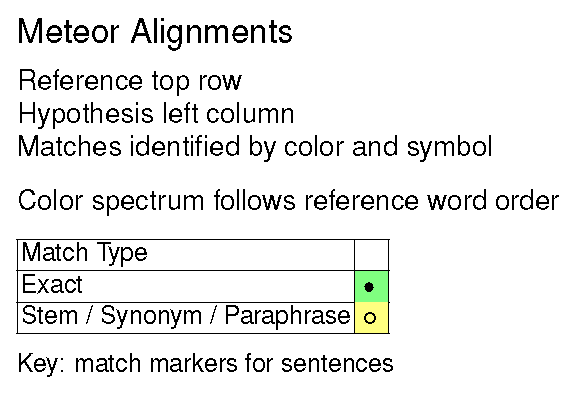
\includegraphics[width=0.25\textwidth]{meteor_alignment_key}
  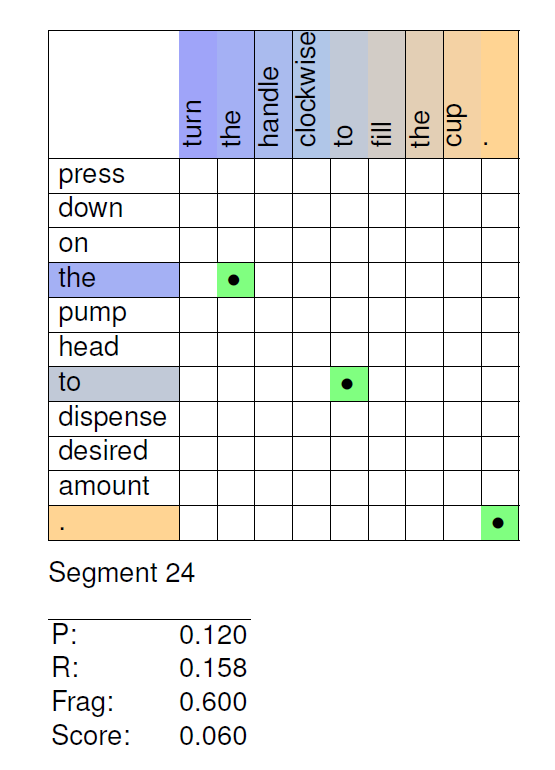
\includegraphics[width=0.25\textwidth]{baseline_seg_24}
  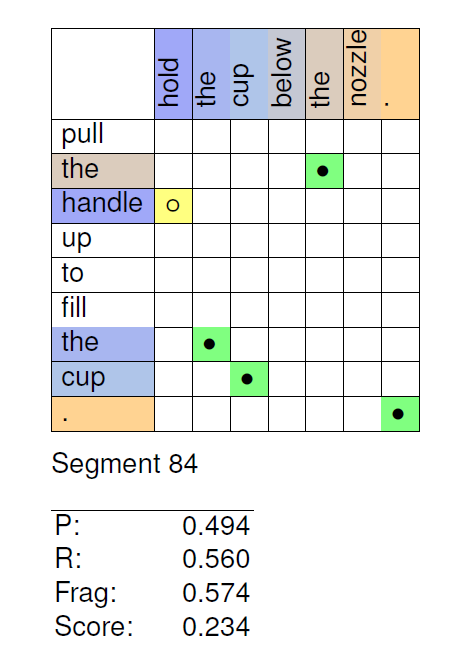
\includegraphics[width=0.25\textwidth]{baseline_seg_84}
  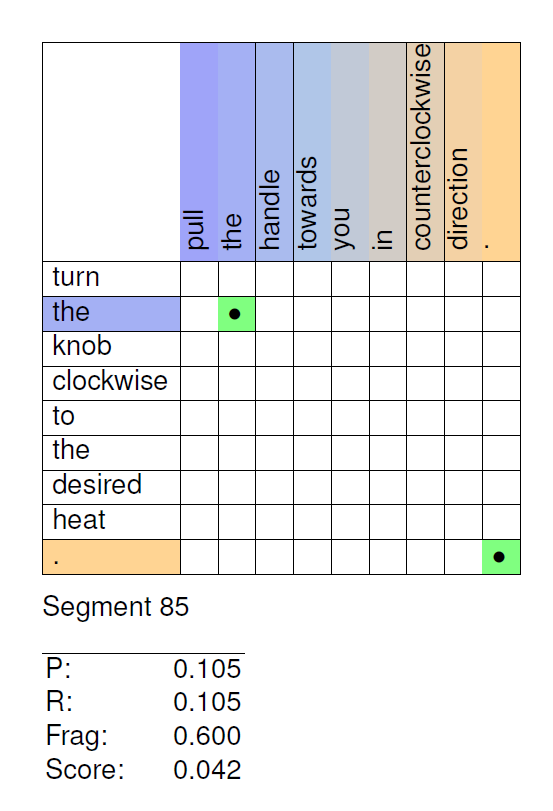
\includegraphics[width=0.25\textwidth]{baseline_seg_85}
  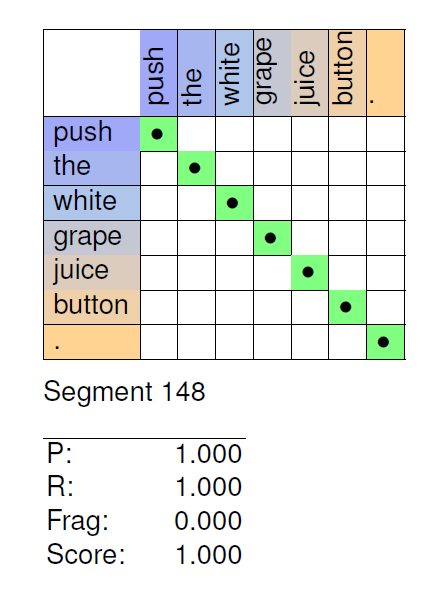
\includegraphics[width=0.25\textwidth]{baseline_seg_148}
  \caption{METEOR alignment for the point-cloud only baseline on Fold 1 segments (i.e. phrases) 24, 84, 85, and 164.}
  \label{fig:baseline_fold_1}
\end{figure}

\begin{figure}[htb!]
  \centering
  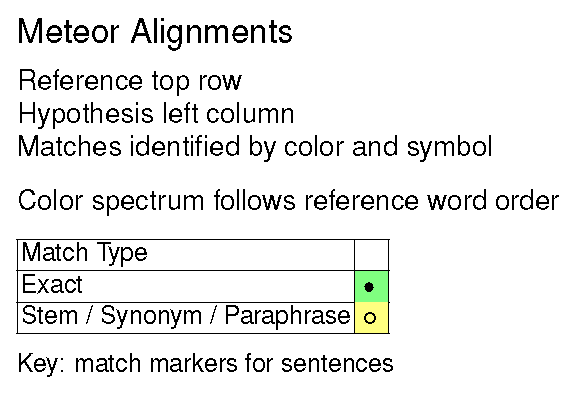
\includegraphics[width=0.25\textwidth]{meteor_alignment_key}
  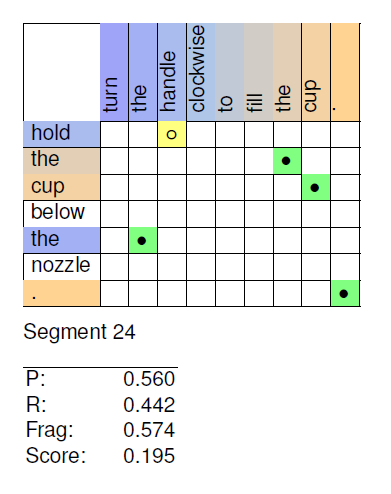
\includegraphics[width=0.25\textwidth]{baseline_w_traj_seg_24}
  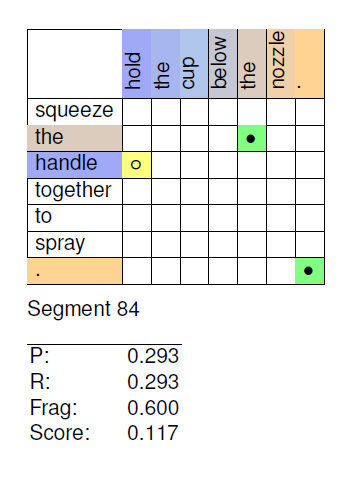
\includegraphics[width=0.25\textwidth]{baseline_w_traj_seg_84}
  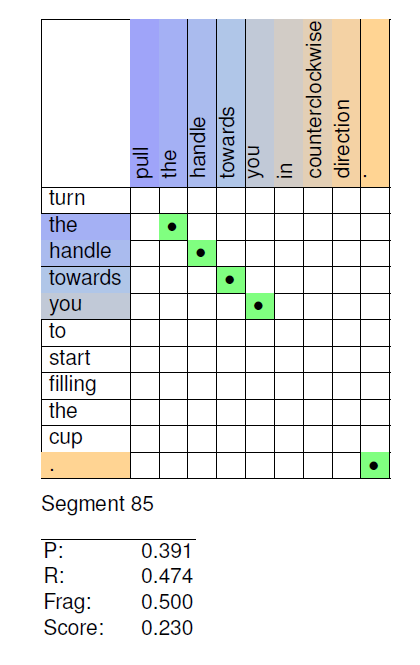
\includegraphics[width=0.25\textwidth]{baseline_w_traj_seg_85}
  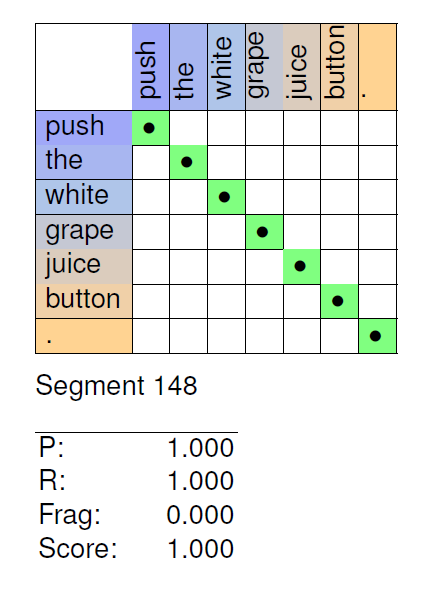
\includegraphics[width=0.25\textwidth]{baseline_w_traj_seg_148}
  \caption{METEOR alignment for the baseline with both point-clouds and trajectories on Fold 1 segments (i.e. phrases) 24, 84, 85, and 164.}
  \label{fig:baseline_w_traj_fold_1}
\end{figure}

\begin{figure}[h]
\centering
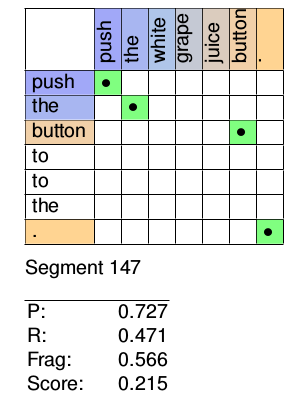
\includegraphics[scale=0.35]{lstm_alignment}
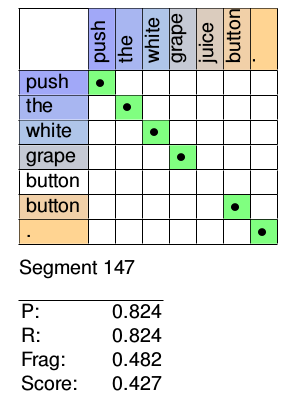
\includegraphics[scale=0.35]{multimodal_lstm_grape}
\caption{METEOR alignment for LSTM performance on Fold 1 segment 147. $Left)$ The unimodal trajectory LSTM. $Right)$ The multimodal, trajectory and point-cloud, LSTM.} 
\label{fig:lstm_alignment}
\end{figure}

\begin{figure}[htb!]
  \centering
  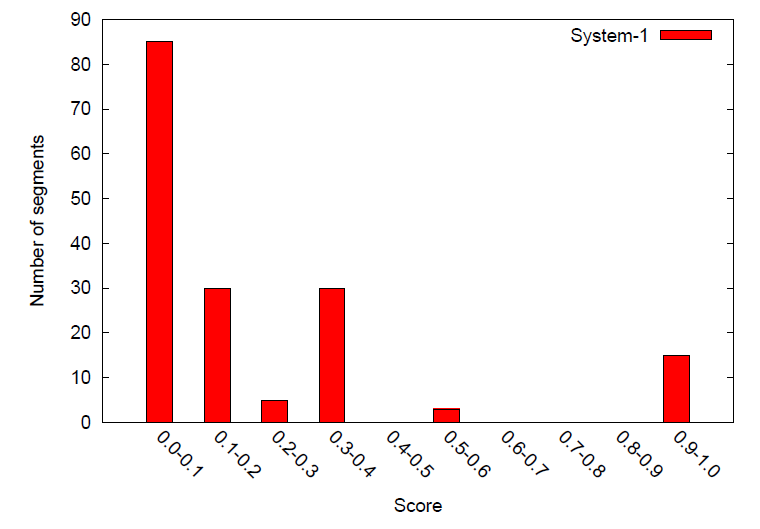
\includegraphics[width=0.45\textwidth]{baseline_score}
  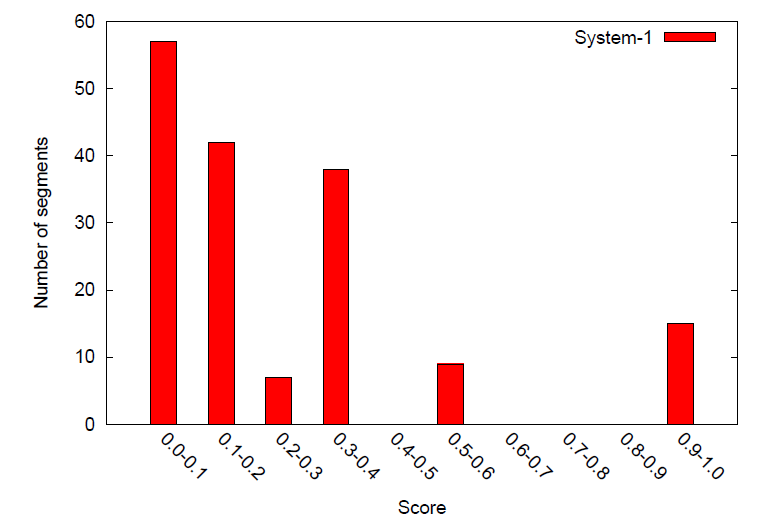
\includegraphics[width=0.45\textwidth]{baseline_w_traj_score}
  \caption{Segment distributions per score ranges for the point-cloud only baseline (left) and baseline with trajectories and point-clouds (right) models on the first fold of data.}
  \label{fig:baselines_fold_1_score}
\end{figure}

\begin{figure}[htb!]
  \centering
  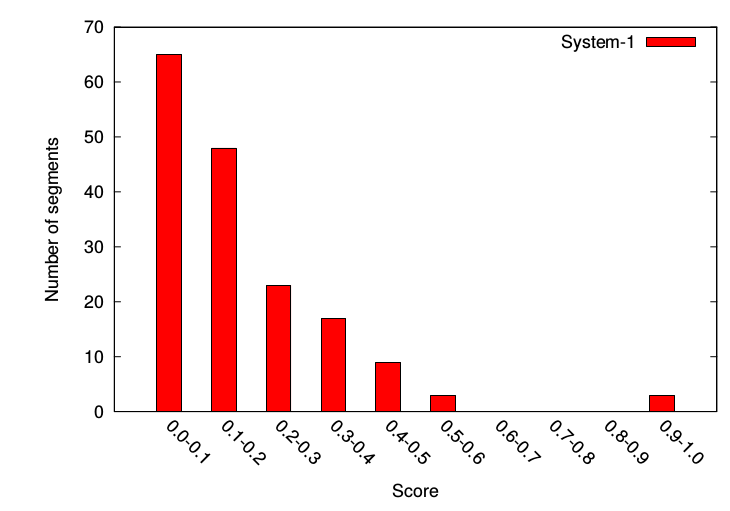
\includegraphics[width=0.45\textwidth]{lstm_fold_1_score_bar_graph}
  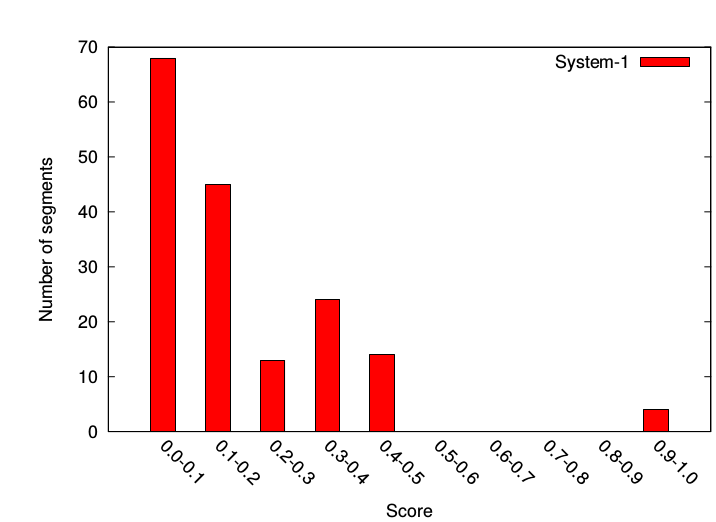
\includegraphics[width=0.45\textwidth]{multimodal_lstm_results}
  \caption{Segment distributions per score ranges for the unimodal LSTM (left) and multimodal LSTM (right) models on the first fold of data.}
  \label{fig:fold_1_score_lstms}
\end{figure}


\end{document}
